\documentclass[pdflatex,11pt]{aghdpl}
% \documentclass{aghdpl}               % przy kompilacji programem latex
% \documentclass[pdflatex,en]{aghdpl}  % praca w języku angielskim
\usepackage[polish]{babel}
\usepackage[utf8]{inputenc}

% dodatkowe pakiety
\usepackage{enumerate}
\usepackage{listings}
\usepackage{graphicx}
\usepackage{url}
\lstloadlanguages{TeX}

\lstset{
  literate={ą}{{\k{a}}}1
           {ć}{{\'c}}1
           {ę}{{\k{e}}}1
           {ó}{{\'o}}1
           {ń}{{\'n}}1
           {ł}{{\l{}}}1
           {ś}{{\'s}}1
           {ź}{{\'z}}1
           {ż}{{\.z}}1
           {Ą}{{\k{A}}}1
           {Ć}{{\'C}}1
           {Ę}{{\k{E}}}1
           {Ó}{{\'O}}1
           {Ń}{{\'N}}1
           {Ł}{{\L{}}}1
           {Ś}{{\'S}}1
           {Ź}{{\'Z}}1
           {Ż}{{\.Z}}1
}

%---------------------------------------------------------------------------

\author{Adam Rzepka}
\shortauthor{A. Rzepka}

\titlePL{Analiza możliwości wykorzystania nowych technologii zawartych w HTML5 do realizacji gry typu FPS}
\titleEN{Analysis}

\shorttitlePL{Analiza} % skrócona wersja tytułu jeśli jest bardzo długi
\shorttitleEN{Analysis}

\thesistypePL{Praca magisterska}
\thesistypeEN{Master of Science Thesis}

\supervisorPL{dr inż. Grzegorz Rogus}
\supervisorEN{Grzegorz Rogus Ph.D}

\date{2013}

\departmentPL{Katedra Informatyki Stosowanej}
\departmentEN{Department of Applied Computer Science}

\facultyPL{Wydział Elektrotechniki, Automatyki, Informatyki i Inżynierii Biomedycznej}
\facultyEN{Faculty of Electrical Engineering, Automatics, Computer Science and Biomedical Engineering}

\acknowledgements{podziękowania}




\setlength{\cftsecnumwidth}{10mm}

%---------------------------------------------------------------------------

\begin{document}

\titlepages

\tableofcontents
\clearpage

\chapter{Wprowadzenie}
\label{cha:wprowadzenie}

%---------------------------------------------------------------------------

\section{Cele pracy}
\label{sec:celePracy}

% ---------------------------------------------------------------------------

\section{Teza pracy}
\label{sec:teza}

\section{Zawartość pracy}
\label{sec:zawartoscPracy}



















%%% Local Variables: 
%%% mode: latex
%%% TeX-master: "praca"
%%% End: 

\chapter{Omówienie dziedziny}
\label{cha:omowienieDziedziny}

\section{HTML5}
\label{sec:html5}
HTML5 jest kolejną wersją języka HTML służącego to tworzenia stron WWW,
opracowywany przez World Wide Web Consortium (W3C) i Web Hypertext Application
Technology Working Group (WHATWG). Standard jest w większości ukończony i jego ostateczna
specyfikacja ma być wydana do końca roku 2014, natomiast w ciągu kolejnych dwóch lat
ma nastąpić wydanie wersji 5.1. Jest on pomyślany jak następca HTML 4.1 i XHTML 1.0.

HTML5 wprowadza wiele nowych tagów (np. canvas, video, audio) oraz interfejsów programistycznych
wymienionych w dalszych podrozdziałach. 
Wraz z nowymi możliwościami HTML5 wraz z językiem JavaScript, stał się platformą
umożliwiającą tworzenie rozbudowanych aplikacji oraz gier.

\begin{figure}[h]
  \centering
  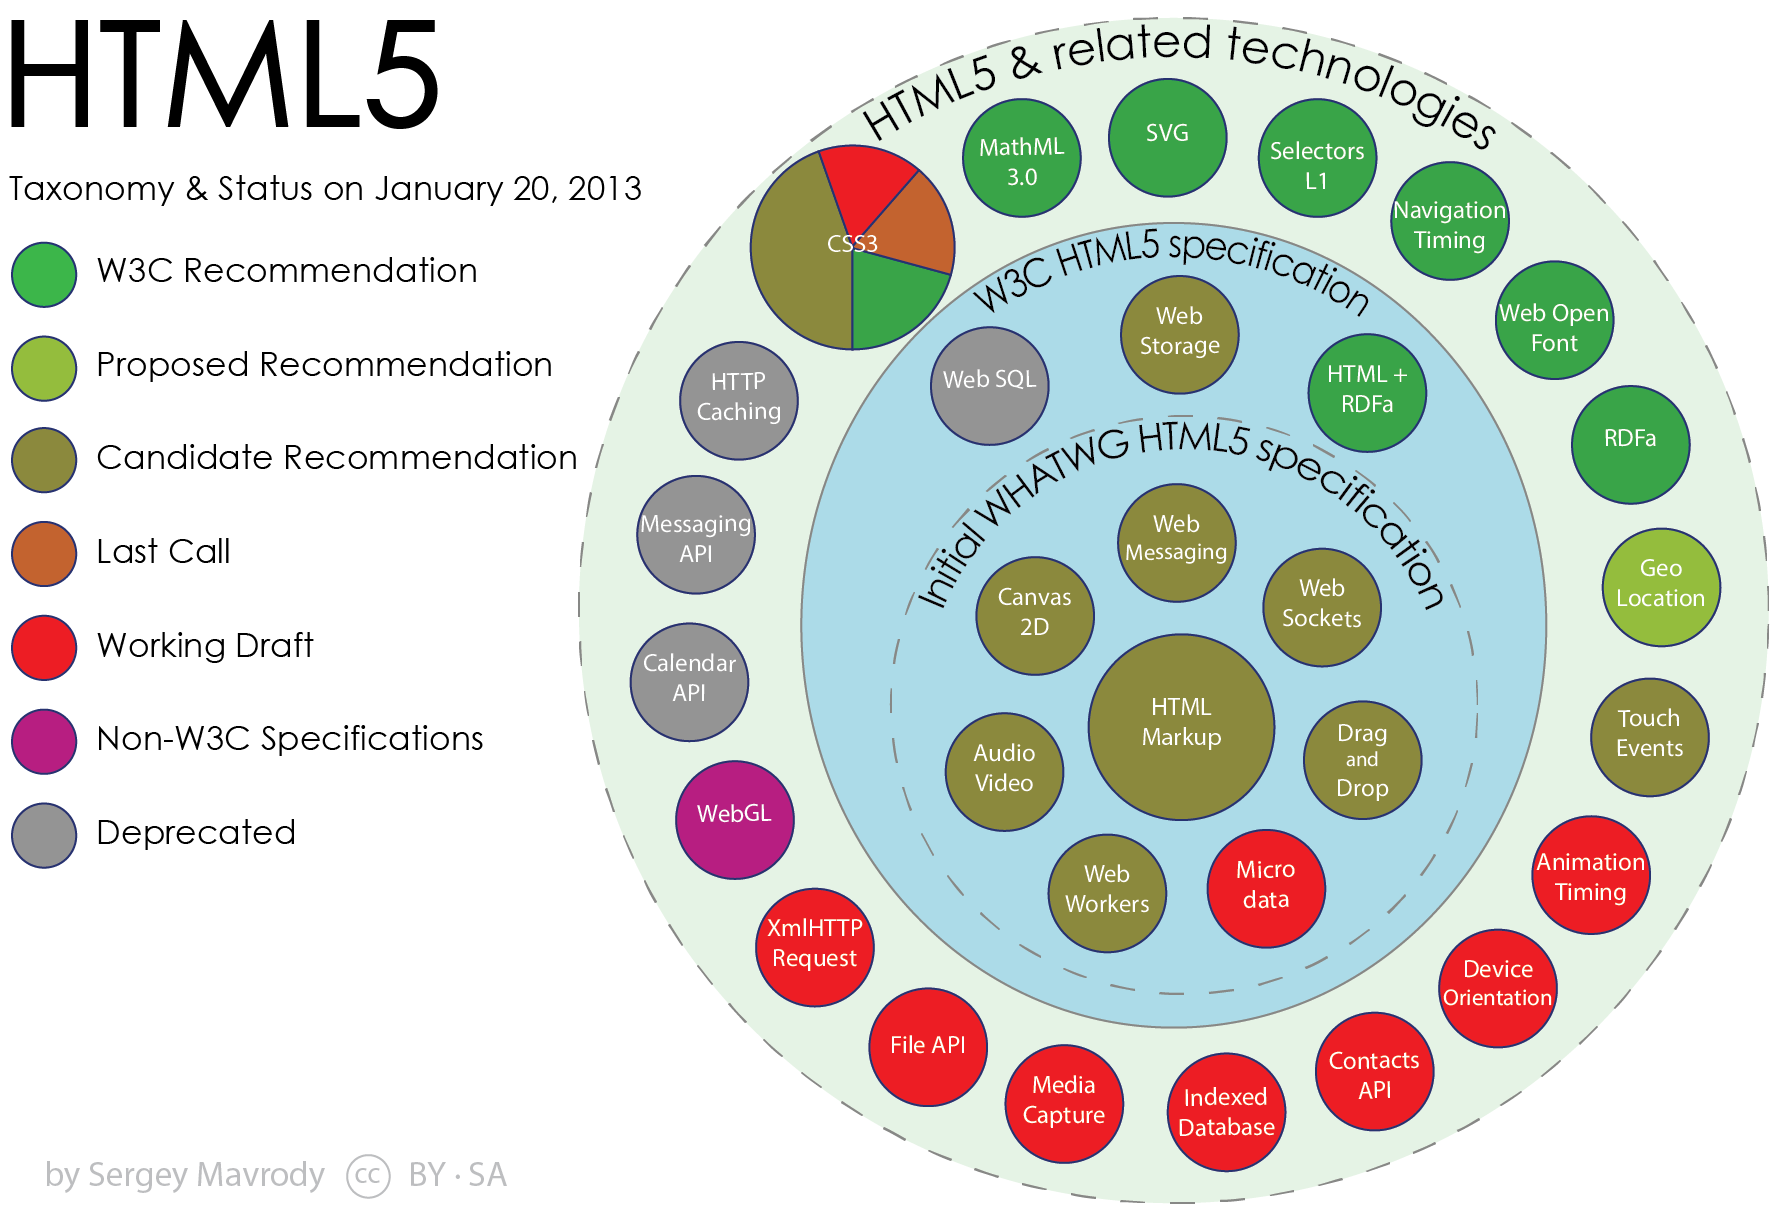
\includegraphics[scale=0.25]{zasoby/rozdzial2/HTML5}  
  \caption{HTML5 i związane z nim technologie oraz ich status.}
  \label{fig:HTML5}
\end{figure}

Pełna specyfikacja HTML5 znajduje się w \cite{html5-spec}.

\subsection{JavaScript}
\label{ssec:javascript}

JavaScript jest skryptowym językiem programowania osadzony w przeglądarkach internetowych
i wykorzystywany do tworzenia interaktywnych stron oraz aplikacji internetowych.
Formalnie nie jest związany z HTML5, jednak jest jedynym językiem obsługiwanym przez
wszystkie przeglądarki, dlatego wszystkie wymienione w dalszych podrozdziałach
interfejsy programistyczne są stworzone dla tego języka.

JavaScript powstał 1995 w firmie Netscape, a następnie został ustandaryzowany przez ECMA (stąd
stosowana formalnie nazwa ECMAScript). Nazwa i składnia przypomina Javę, jednak jest to podobieństwo
mylące. JavaScript jest językiem dynamicznym, posiadającym wiele cech języków funkcyjnych,
a obiektowość jest oparta na prototypach, a nie klasach. Specyfikacja języka ECMAScript jest
publicznie dostępna na stronie \cite{ecma-spec}, natomiast wyczerpujące wprowadzenie można
znaleźć w \cite{js-definitive}.

Początkowo JavaScript był używany do wyświetlania prostych animacji,
komunikatów i wstępnej walidacji danych w formularzach. Z w JavaScripcie czasem zaczęły
powstawać coraz bardziej rozbudowane aplikacje i okazało się, że wydajność interpretowanego
języka skryptowego z Garbage Collectorem (odśmiecaczem) jest coraz większym problemem.
Rozpoczął się wyścig pomiędzy twórcami
przeglądarek o jak najszybszy silnik skryptowy. W rezultacie, obecnie w większości przeglądarek
skrypty są kompilowane do kodu natywnego przez kompilator JIT (Just In Time), z zastosowaniem wielu
technik optymalizacji kodu, a Garbage Collector jest coraz szybszy. Dostępne są również
rozbudowane narzędzia do profilowania kodu JavaScript.

Ta sytuacja sprawiła, że JavaScript zaczął się nadawać do robienia wymagających obliczeniowo
gier 3d. Oczywiście wciąż trzeba unikać szczególnie nieefektywnych konstrukcji tego języka
i starać się alokować jak najmniej obiektów, aby ograniczyć przestoje powodowane przez działanie
odśmiecacza. Jednak przy zachowaniu tych zasad, wydajność współczesnych silników JavaScript
powinna być wystarczająca dla wielu gier.


\subsubsection{asm.js}
\label{sec:asmjs}

asm.js jest to podzbiór JavaScript opracowany przez Mozillę, który zapewnia najszybsze wykonanie.
Programowanie zgodnie z asm.js jest jednak bardzo żmudne, dlatego podzbiór ten jest głównie
pomyślany jak cel kompilatorów innych języków do JavaScript (np. Emscripten [link/footnote]). Nie istnieje
obecnie translator dowolnego kodu JavaScript do asm.js. Ponieważ gra będąca przedmiotem niniejszej
pracy powstaje w JavaScript, tematyka asm.js nie będzie szerzej omawiana. Więcej informacji można
znaleźć na stronie internetowej \cite{asm-js}.

\subsection{WebGL}
\label{ssec:webgl}

WebGL jest to API dla języka JavaScript służące do wyświetlania grafiki 3d w przeglądarce.
Z tego powodu jest to najbardziej istotna technologia z punktu widzenia
twórców gier. Pomimo, że formalnie WebGL nie jest jeszcze
częścią standardu HTML5, to jest on zaimplementowany we wszystkich znaczących
przeglądarkach.

WebGL bazuje na standardzie OpenGL ES 2.0 (Open Graphics Library for
Embedded Systems) przeznaczonym dla urządzeń mobilnych, który z kolei
jest uproszczoną wersją OpenGL (Open Graphics Library) -- otwartego API do
renderowania grafiki 3d, będącym jednym z dwóch (obok Direct3D) szeroko
stosowanych API do wyświetlania grafiki w grach i programach wykorzystujących 3d.
Wszystkie te standardy zostały opracowane przez konsorcjum Khronos Group (wcześniej ARB),
zrzeszające wszystkie (poza Microsoftem) większe firmy zainteresowane tematem grafiki 3d.

Prace nad WebGL rozpoczęła Mozilla w 2006 roku. A w następnym roku Firefox oraz Opera
miały już pierwsze działające implementacje. Były one kontynuowane w grupie roboczej
WebGL Working Group działającej w ramach Khronos Group z udziałem m. in. Mozilli,
Opery, Google oraz Apple. W 2011 roku ukończona została pierwsza wersja standardu, a w 2013
ruszyły prace nad wersją 2.0 bazującą na OpenGL 3.0. W tym też roku Microsoft wydał
Internet Explorer 11 z obsługą WebGL, pomimo początkowej niechęci do tego standardu
(Microsoft promuje swoją technologię Direct3D, konkurencyjną w stosunku do OpenGL).
Tym samym ostatnia z liczących się przeglądarek dodała obsługę WebGL.

WebGL zaprojektowano dla języka JavaScript, w przeciwieństwie do OpenGL i OpenGL ES,
które przeznaczone są głównie dla języka C. Jednakże jest interfejsem bardzo
niskopoziomowym, w zasadzie dokładnie przełożonym na JavaScript OpenGL ES. Dodano
jedynie kilka usprawnień (jak wczytywanie tekstury z elementu HTML <img>) oraz
dodatkową walidację danych, istotną w środowisku tekstowym. Z tego powodu programiści
JavaScript mogą uznać API za trudne i nieprzystępne. Z drugiej jednak strony, taka
implementacja gwarantuje maksymalną szybkość działania, a programiści znający OpenGL mogą
w zasadzie natychmiast zacząć używać WebGL. Specyfikacja WebGL znajduje się na stronie
\cite{webgl}.


\subsection{Web Workers}
\label{ssec:webWorkers}

Współcześnie każdy domowy komputer posiada wielordzeniowy procesor. W tym samym kierunku
podążają procesory w urządzeniach mobilnych. Aby maksymalnie wykorzystać moc obliczeniową,
konieczne jest tworzenie aplikacji współbieżnych. Niestety JavaScript przez długi czas
tego nie umożliwiał. Zmienia to API Web Workers należące do standardu HTML5.

Worker jest to odpowiednik wątku dla języka JavaScript. Jednakże jego sposób działania
upodabnia go bardziej do procesu -- poszczególne workery nie mogą współdzielić pamięci
i komunikują się wyłącznie za pomocą wysyłanych wiadomości. Dzięki takiej konstrukcji
można uniknąć wielu problemów związanych z klasyczną wielowątkowością, jednak odbywa
się to kosztem wydajności z powodu konieczności częstego kopiowania danych. Dodatkowo
API dostępne dla workera jest bardzo ograniczone (np. nie ma dostępu do elementów HTML).

Te cechy powodują, że aby osiągnąć zysk wydajnościowy przy pomocy Web Workers, trzeba od
początku projektować aplikację pod kątem tego API -- tak aby ograniczyć ilość przesyłanych
danych.

Należy zaznaczyć, iż taki sposób tworzenia aplikacji wielowątkowych jest nieobcy programistom
gier, gdyż podobny model wymuszał procesor Cell w konsoli PlayStation3. Procesor ten składa
się z jednego głównego rdzenia (tzw. Power Processing Element) oraz kilku rdzeni wspomagających
(tzw. Synergistic Processing Element), które również nie mogą współdzielić pamięci. Podobnie jak
Web Workerze, tak w programie działającym na SPE, dostępne API jest bardzo ograniczone.

\subsection{Web Sockets}
\label{ssec:webSockets}

Wiele współczesnych gier umożliwia wspólną rywalizację wielu graczy za pośrednictwem internetu
(tzw. multiplayer). W celu implementacji gry sieciowej konieczne jest API do komunikacji
internetowej.

Interfejs Web Sockets jest odpowiednikiem systemowych gniazd sieciowych i umożliwia komunikację
w czasie rzeczywistym pomiędzy aplikacją JavaScript, a serwerem za pośrednictwem protokołu TCP.
Jest on częścią HTML5 i dostępny we wszystkich znaczących przeglądarkach.

\subsection{WebRTC}
\label{ssec:webrtc}

Wprowadzenie interfejsu Web Sockets było istotnym krokiem z punktu widzenia twórców gier
sieciowych, ma on jednak pewne ograniczenia. Jest oparty o protokół TCP, którego 
niezawodność powoduje opóźnienia w transmisji danych (przesyłanie potwierdzeń,
retransmisje itp.). Dodatkowo cały ruch musi być kierowany przez serwer, gdyż bezpośrednia
komunikacja pomiędzy przeglądarkami jest niemożliwa. To sprawia, że Web Sockets nie nadają
się do bardzo dynamicznych gier.

Rozwiązanie tego problemu nadeszło ze strony interfejsu WebRTC (od Real Time Communication),
mającego służyć przede wszystkim
do przesyłanie wideo i dźwięku w czasie rzeczywistym pomiędzy przeglądarkami, dzięki czemu
możliwe byłoby zbudowanie komunikatora wideo w przeglądarce.

WebRTC umożliwia również przesyłanie dowolnych danych tekstowych i binarnych, a ponieważ
działa w oparciu o protokół UDP i łączy bezpośrednio przeglądarki (peer-to-peer), idealnie
nadaje się do szybkich gier sieciowych. Oczywiście użycie  bezpołączeniowego protokołu UDP
powoduje, że aplikacja sama musi zapewnić poprawność działania w przypadku błędów przesyłu. 

WebRTC był początkowo tworzonym przez Google, lecz wkrótce prace przejęła grupa robocza w W3C,
złożona m.in. z Google, Mozilli i Opery. Niestety Microsoft odmówił wsparcia dla WebRTC i  -- jak
to miało miejsce już wielokrotnie -- zaczął tworzyć swój alternatywny standard: CU-RTC-WEB
(Customizable, Ubiquitous Real-Time Communication over the Web). Dlatego WebRTC nie jest
obsługiwany w Internet Explorer i nie ma żadnych planów jego implementacji. Co więcej,
żadna z przeglądarek nie posiada jeszcze pełnej i stabilnej implementacji (stan na
początek 2014 roku). Jednakże w niektórych (Chrome, Firefox) API już na tyle dojrzało, że
można go z powodzeniem używać.

\subsection{Web Audio API}
\label{ssec:webAudio}

Poza grafiką, w grach bardzo ważna jest również oprawa dźwiękowa. O ile odtwarzanie muzyki
nie było problemem od czasu wprowadzenia taga <audio> to udźwiękowienie efektów w grze
wymagało bardziej zaawansowanego API.

W tym celu do HTML5 zostało wprowadzone Web Audio API. Jest to wysokopoziomowy, zaawansowany
interfejs do przetwarzania i odtwarzania dźwięków w JavaScript. Umożliwia on wszystko co
potrzebne do udźwiękowienia gry -- dźwięk przestrzenny, nakładanie wielu efektów itp.

Aktualnie (2014) Web Audio API jest wspierane przez wszystkie większe przeglądarki oprócz
Internet Explorer.

\subsection{Pozostałe przydatne API}
\label{ssec:pozostaleApi}

HTML5 zapewnia wiele interfejsów programistycznych przydatnych w wielu aplikacjach
i grach w zależności od potrzeb. Wśród bardziej przydatnych należałoby wymienić:
\begin{itemize}
\item Gamepad API -- obsługa gamepadów, joysticków, kierownic komputerowych itp.
\item Mouse Lock API -- możliwość ukrycia i zablokowania kursora myszy,
\item Fullscreen API
\item Web Storage -- przechowywanie danych po stronie klienta (np. w celu cache'owania danych gry),
\item File API -- operowanie na plikach,
\item XmlHTTPRequest -- asynchroniczne pobieranie plików z serwera (standard de facto
  od dłuższego czasu),
\item Device Orientation i Touch Events -- dla urządzeń mobilnych.
\end{itemize}

%%%%%%%%%%%%%%%%%%%%%%%%%%%%%%%%%%%%%%%%%%%%%%%%%%%%%%%%%%%%%%%%%%%%%%%%%%%%%%%%

\section{Gry Komputerowe}
\label{sec:gryKomputerowe}

Gry komputerowe to w dzisiejszych czasach ogromny rynek zapewniający rozrywkę milionom graczy
na całym świecie. Historia gier zaczęła się niedługo po wynalezieniu komputerów. Początkowo
były to bardzo proste programy, jednak z czasem stawały się coraz bardziej skomplikowane,
zarówno pod względem technicznym (grafika, dźwięk), jak i pod względem mechaniki (zasad gry).

\begin{figure}[h]
  \centering
  
\includegraphics[scale=0.5]{zasoby/rozdzial2/mario}  
  \caption{Jedna z najsłynniejszych gier w historii -- Super Mario Bros.}
  \label{fig:mario}
\end{figure}

Gry opanowały wiele platform sprzętowych. Wcześniej utożsamiane głównie z automatami i konsolami,
wkrótce odniosły wielki sukces na komputerach osobistych,
a współcześnie na telefonach i tabletach.
Co prawda gry działające w przeglądarce pojawiały się od początku istnienia języka JavaScript,
czy platformy Adobe Flash (wcześniej Macromedia Flash), jednak były one utożsamiane
z bardzo prostą rozgrywką i ubogą warstwą audiowizualną. Wraz w nadejściem ery HTML5
i technologii z nim związanych (przede wszystkim WebGL), zaistniała możliwość ekspansji
bardziej zaawansowanych gier na ten -- stosunkowo jeszcze młody -- rynek.

Zainteresowani tematyką tworzenia gier znajdą obszerne wprowadzenie w \cite{game-engine}.

W następnych podrozdziałach zostanie przedstawiony gatunek gier FPS oraz dwie gry tego typu,
szczególnie związane z niniejszym opracowaniem, a także silnik gry, na którym są oparte.
Następnie wprowadzone zostaną koncepcje związane z architekturą gier sieciowych (mutliplayer).

\subsection{Gry FPS}

Przedmiotem pracy jest stworzenie gry typu FPS działającej w przeglądarce. 

Skrót FPS oznacza First Person Shooter. Jest to strzelanina w której obserwujemy świat
oczami bohatera. Gry typu FPS należą do najstarszych i najczęściej występujących gier
3d. Z jednej strony mają one dość prostą mechanikę i zasady, z drugiej natomiast, często
są bardzo zaawansowane technologicznie i bywają pionierskie w dziedzinach takich jak
realistyczna grafika, czy rozgrywka sieciowa. Dlatego właśnie taki gatunek został wybrany
do implementacji w HTML5.

\begin{figure}[h]
  \centering
  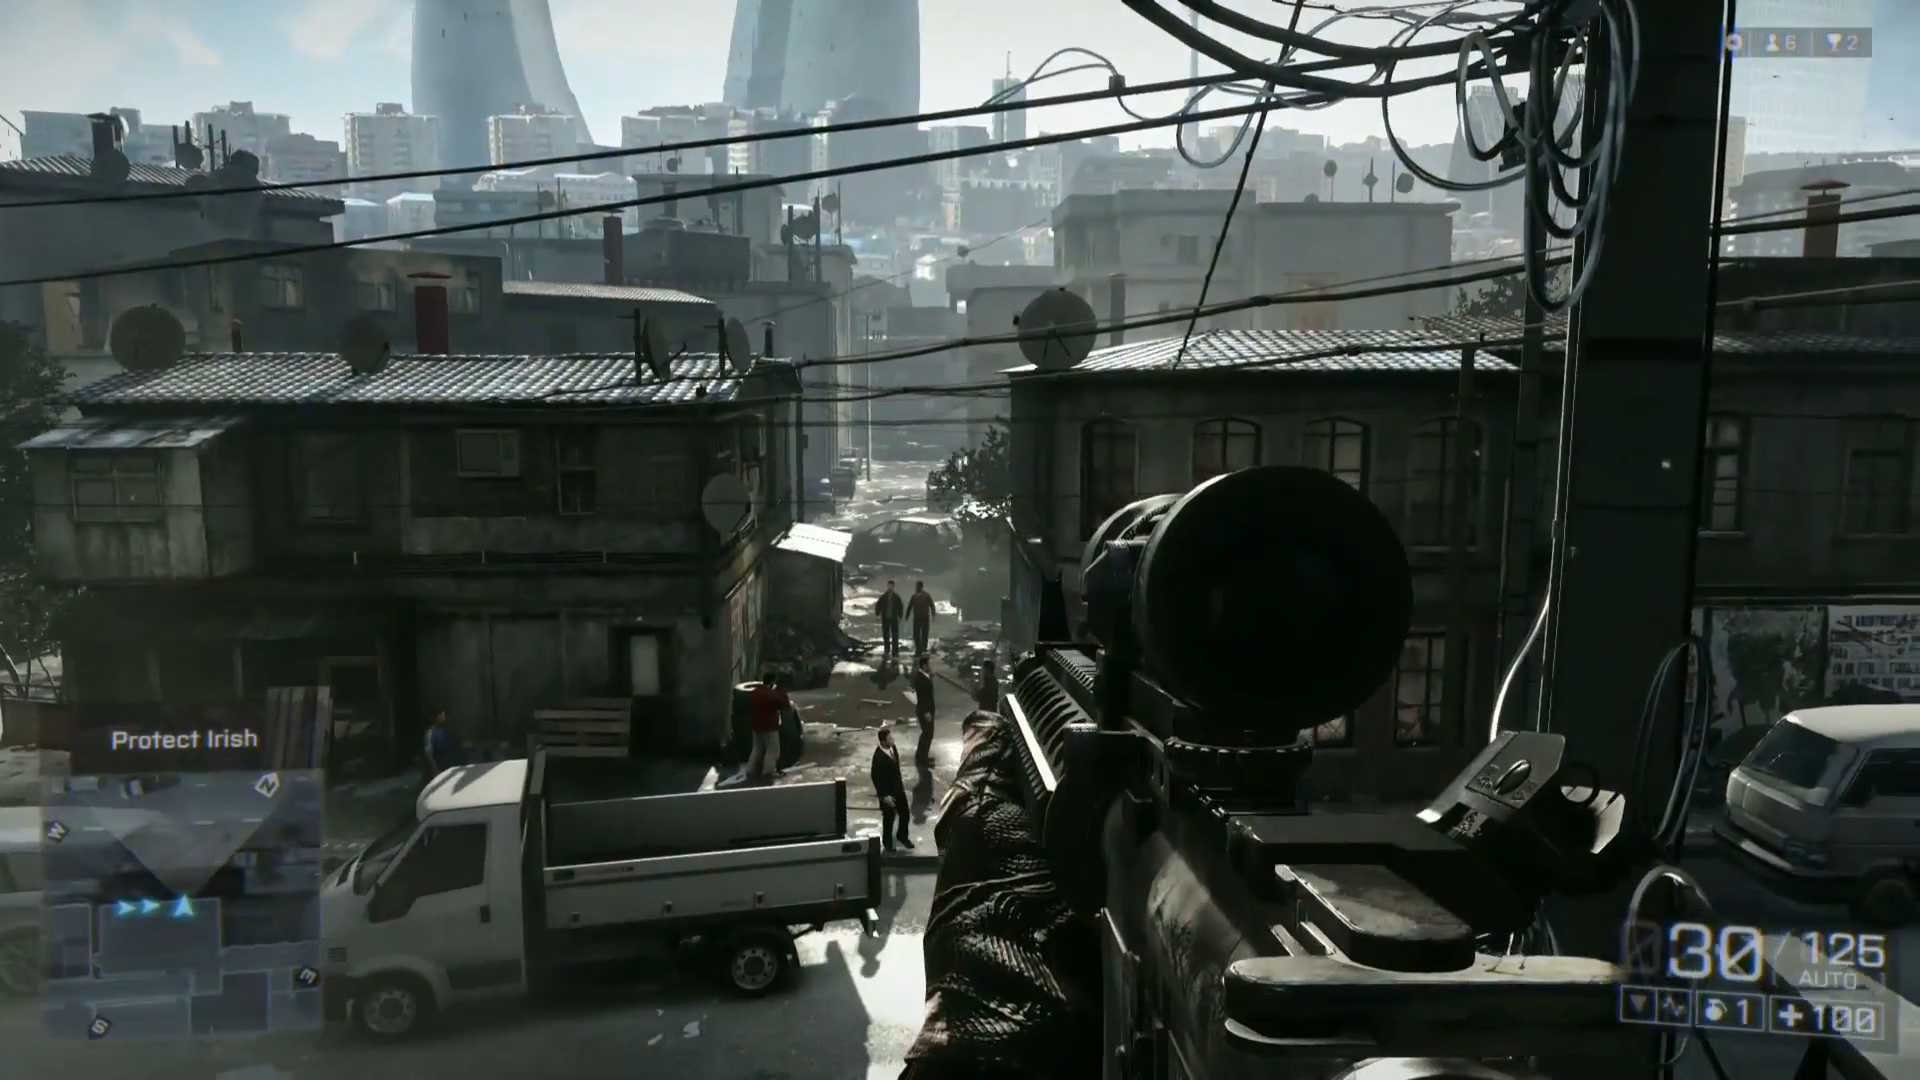
\includegraphics[scale=0.25]{zasoby/rozdzial2/battlefield4}  
  \caption{Współczesna gra FPS -- Battlefield 4}
  \label{fig:battlefield4}
\end{figure}

\subsection{Quake III Arena}
\label{ssec:quake3}

W roku 1996 ukazała się gra Quake, która odniosła wielki sukces, głównie dzięki
rewolucyjnej grafice i dopracowanej rozgrywce sieciowej. Twórcą gry była firma
id Software. Rok później powstała kolejna część - Quake II.

Z racji ogromnej popularności trybu dla wielu graczy, kolejna część -- Quake III
Arena -- zupełnie porzuciła tradycyjny tryb fabularny i skupiła się tylko na
rozgrywce sieciowej. Została wydana w roku 1999.
Gra również odniosła sukces i do dziś pozostaje popularna
pośród graczy. Profesjonalne turnieje gier sieciowych (tzw. e-sport) bardzo
często w swoim programie mają rozgrywki w Quake III Arena.
W roku 2000 ukazał się dodatek do gry pod nazwą Quake III Team Arena.
\begin{figure}[h]
  \centering
  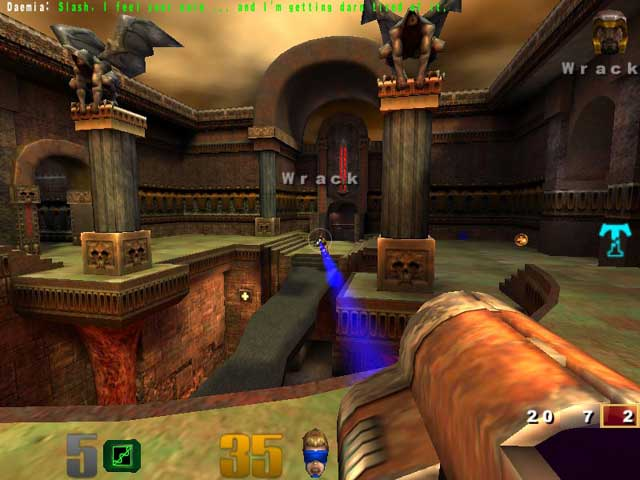
\includegraphics[scale=0.5]{zasoby/rozdzial2/quake3}  
  \caption{Scena z gry Quake III Arena}
  \label{fig:quake3}
\end{figure}

Siedem lat później, w roku 2007 id Software rozpoczął prace nad wydaniem
Quake III Arena i Team Arena na przeglądarki internetowe pod nazwą Quake Live.
Kod gry uruchamiany był poprzez specjalnie stworzoną wtyczkę do
przeglądarki. W związku z tym rozgrywka była możliwa tylko na wybranych systemach
operacyjnych i przeglądarkach, konieczna też była instalacja wtyczki przez
gracza.

w międzyczasie, w roku 2005 ukazał się Quake IV, który kontynuował wątki fabularne
z Quake II. Gra pomimo dobrych ocen w prasie nie przyjęła się tak dobrze
wśród graczy, głównie ze względu na brak znaczących ulepszeń w trybie sieciowym.

Quake III oraz Quake Live jest oparty na silniku gry o nazwie id Tech 3, o którym
będzie mowa w podrozdziale \ref{ssec:idTech}.

\subsection{OpenArena}
\label{ssec:openArena}

W roku 2005 główny programista id Software, John Carmack, ogłosił uwolnienie
kodu źródłowego silnika id Tech 3 na licencji GNU GPL. Uwalnianie źródeł swoich
starszych technologii jest już tradycją w tej firmie.

Wkrótce rozpoczęły się prace nad wieloma grami open source korzystającymi
z tego silnika. Jedną z najbardziej dojrzałych jest OpenArena.

OpenArena jest właściwie klonem Quake III Arena. Ponieważ z pierwowzoru został
udostępniony tylko kod, fani utworzyli potrzebne zasoby gry (modele, tekstury itp.),
również na licencji GPL. Wprowadzono też wiele usprawnień do kodu gry,
dodając np. obsługę nowszej wersji OpenGL i shaderów \footnote{Shader - niewielki program
  działający na karcie graficznej, opisujący właściwości wierzchołków
  i pikseli.}. Tym samym OpenArena stała się pełnoprawną
i całkowicie otwartą grą.

Grę OpenArena można pobrać ze strony \url{http://openarena.ws/}.

\subsection{id Tech 3}
\label{ssec:idTech}

Każda bardziej zaawansowana gra posiada w kodzie źródłowym mniej lub bardziej
rozgraniczony rdzeń nazywany silnikiem gry. Odpowiada on za wczytywanie
i wyświetlanie świata 3d, odtwarzanie dźwięków, obsługę sieci oraz wiele
innych zadań. Często jeden silnik jest wykorzystywany przy tworzeniu wielu gier.

id Software zawsze wykorzystywało swoje autorskie silniki, których źródła były
publikowane po utworzeniu nowej wersji. Quake III Arena, a potem OpenArena
wykorzystywały id Tech w wersji 3.

Silnik ten był bardzo zaawansowany technologicznie jak na swoje czasy. Do wyświetlania
grafiki konieczny był sprzętowy akcelerator graficzny. Pośród ciekawszych
możliwości tego silnika należy wymienić:
\begin{itemize}
\item wyświetlanie powierzchni opartych na krzywych sklejanych,
\item system tzw. skryptów shaderów, dzięki którym graficy mieli dużą kontrolę
  nad wyglądem każdej powierzchni \footnote {Nie należy mylić tego systemu nieistniejącymi
    jeszcze shaderami działającymi na karcie graficznej. Skrypty z id Tech3 były jednak pewną
    namiastką shaderów w dzisiejszym rozumieniu.},
\item wyświetlanie generowanych wcześniej map oświetlenia, zapewniających bardziej
  realistyczny wygląd otoczenia,
\item przestrzenna mgła,
\item odbicia lustrzane,
\item zaawansowany system synchronizacji stanu gry przez sieć,
\item QVM -- wbudowana wirtualna maszyna wykonująca kod gry.
\end{itemize}

Interesujące omówienie architektury silnika id Tech 3 znajduje się w \cite{q3-code-reviev}.

\subsection{Multiplayer}
\label{ssec:multiplayer}

Multiplayer jest to tryb gry, w którym uczestniczy wielu graczy, zazwyczaj za
pośrednictwem Internetu. Tryb ten jest często spotykany w grach FPS, ale także
w grach wyścigowych, czy strategiach. Wiele gier i graczy skupia się wyłącznie
na grze sieciowej. Zdarza się, że w jednej rozgrywce uczestniczy na raz
tysiące graczy \footnote {Są to tak zwane gry MMO -- Massive Multiplayer Online}

Tryb multiplayer wymaga, aby wszyscy gracze widzieli ten sam stan gry.
Synchronizacja gry pomiędzy komputerami w sieci jest zagadnieniem nietrywialnym,
szczególnie w przypadku gier bardzo dynamicznych i posiadających złożoną mechanikę
(a przez to złożony opis stanu gry).

Z punktu widzenia organizacji w sieci, możliwe są dwie architektury:
\begin{itemize}
\item Peer-to-peer -- nie ma głównego komputera, każdy komputer rozsyła do wszystkich
  pozostałych informacje o każdej akcji wykonanej przez gracza lokalnego. Architektura
  ta jest rzadko używana, ze względu na trudność z synchronizacją i problemy z
  nieuczciwymi graczami.
\item Klient - serwer -- najczęściej używana. Jeden z komputerów jest serwerem
  gry. Na nim odbywa się cała symulacja, a wszyscy klienci służą jedynie jako
  terminale, wysyłając informacje o naciśniętych przez gracza przyciskach
  i otrzymując migawkę (snapshot) aktualnego stanu gry do wyrenderowania.
\end {itemize}

Należy zaznaczyć, że serwer niekoniecznie musi być dedykowaną maszyną utrzymywaną
przez producenta gry. W przypadku gier w niewielką liczbą uczestników,
zazwyczaj jeden z komputerów graczy pełni rolę serwera. Dodatkowo, bardzo
często producent zapewnia tzw. lobby server, czyli główny serwer,
który służy m. in. do odnajdywania toczących się właśnie rozgrywek
i inicjalizacji połączenia. W związku z tym pojęcie serwer może mieć
dwa różne znaczenia i wymaga doprecyzowania, dlatego na potrzeby dalszej części pracy
wprowadzimy następujące pojęcia:
\begin{itemize}
\item serwer główny lub lobby -- serwer utrzymywany przez dewelopera, zbierający
  informacje o toczących się grach i ułatwiający inicjalizację połączenia,
\item serwer gry -- instancja gry która zarządza konkretną rozgrywką
\end{itemize}

\begin{figure}[h]
  \centering
  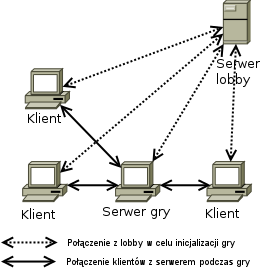
\includegraphics[scale=1]{zasoby/rozdzial2/multiplayer}  
  \caption{Schemat połączeń sieciowych w grze multiplayer typu klient - serwer, jeden z komputerów graczy pełni rolę serwera gry.}
  \label{fig:multiplayer}
\end{figure}

W przypadku gry przeglądarkowej, serwer gry działa w przeglądarce, co może
wprowadzić dodatkowe nieporozumienie, gdyż w aplikacjach webowych przeglądarka
jest tożsama z klientem HTTP.

Zagadnienie programowania gry multiplayer jest bardzo obszerne. Jeden z dokładniejszych
opisów można znaleźć w \cite{algorithms-networking}.

%%%%%%%%%%%%%%%%%%%%%%%%%%%%%%%%%%%%%%%%%%%%%%%%%%%%%%%%%%%%%%%%%%%%%%%%%%%%%%%%

\section{Poprzednie prace}
\label{sec:poprzedniePrace}

W niniejszym rozdziale zaprezentowane zostaną projekty, mające związek z tematyką pracy.

\subsection{Quake II w przeglądarce}
\label{ssec:quake2web}

W roku 2010 dwaj pracownicy Google, Joel Webber i Ray Cromwell
udostępnili swój projekt -- port Quake II
na przeglądarki z wykorzystaniem WebGL. Była to jedna z pierwszych prac,
które udowodniły możliwość zaistnienia gier 3d w przeglądarkach.

quake2-gwt-port, bo tak został nazwany projekt, powstał poprzez skompilowanie
w GWT \footnote{GWT -- Google Web Toolkit -- SDK do tworzenie aplikacji webowych w języku Java,
  posiadające również kompilator części klienckiej do JavaScript.
  \url{http://www.gwtproject.org/} }
kodu Jake2 -- portu Quake II do Javy.
Projekt ten nie powstał bezpośrednio w JavaScript, przez co nie integruje się
zbyt dobrze ze środowiskiem webowym, a do uruchomienia konieczne było
wiele łat i rozwiązań prowizorycznych. Dodatkowo w roku 2010 nie istniało
jeszcze Mouse Lock API, przez co sterowanie grą jest bardzo trudne.

Z tych powodów projekt ten należy uznać raczej za demo technologiczne niż
grę. Mimo to był to ważny krok milowy dla technologii WebGL.

Strona projektu: \url{https://code.google.com/p/quake2-gwt-port/}.

\subsection{Quake III level viewer}
\label{ssec:quake3web}

W tym samym roku Brandon Jones zaprezentował swoje demo o nazwie q3bsp.
Jest to level viewer\footnote{Level viewer - narzędzie umożliwiające
  podgląd danego poziomu gry, bez uruchamiania logiki rozgrywki} poziomów
z Quake III Arena. W przeciwieństwie do quake2-gwt-port, q3bsp został
w całości napisany w JavaScripcie, dzięki czemu mógł użyć wiele udogodnień
zapewnianych przez środowisko przeglądarki (np. zapewnione wczytywanie
plików graficznych, interfejs użytkownika w HTML), a jego wydajność
jest dużo lepsza, pomimo bardziej zaawansowanej grafiki.

Projekt ten również zyskał duży rozgłos w środowisku deweloperów WebGL
i poza nim. Można go zobaczyć na stronie \url{http://media.tojicode.com/q3bsp/}.
Część kodu źródłowego
q3bsp (udostępnionego na licencji zlib) została wykorzystana w niniejszej pracy.

\subsection{Banana Bread}
\label{ssec:bananaBread}

Banana Bread jest portem gry Cube2:Sauerbraten (\url{http://sauerbraten.org/})
na JavaScript zrobionym
przez Mozillę. Powstał przez kompilację z C++ kompilatorem Emscripten.

Jest to pełnoprawna i działająca gra, w którą można zagrać na stronie \url{https://developer.mozilla.org/pl/demos/detail/bananabread}.


%%% Local Variables: 
%%% mode: latex
%%% TeX-master: "praca"
%%% End: 

\chapter{Rozdział do testów}

Brak sensownej zawartości ;)



\chapter{Implementacja}
\label{cha:implementacja}

W niniejszym rozdziale zostanie bardziej szczegółowo opisana realizacja komponentów
gry opisanych w części \ref{cha:projekt}.

\section{Wyjaśnienie dotyczące zamieszczonych diagramów UML}
\label{sec:uml}

W niniejszej części pracy będzie wykorzystywany język UML do przedstawienia implementacji
poszczególnych komponentów. Język ten pomimo swej użyteczności nie jest jednak idealny
do przedstawiania kodu programu stworzonego w JavaScript, dlatego trzeba na początku
wyjaśnić kilka nieścisłości.

UML operuje na pojęciach znanych z języków obiektowych, wykorzystujących klasy. Są to pojęcia
takie jak klasa, interfejs, metoda, dziedziczenie itp. Jednakże w JavaScript obiektowość
jest realizowana przez prototypy\footnote{Więcej na ten temat paradygmatu programowania
  przez prototypowanie w \cite{js-definitive}.}, a więc
terminy te nie występują w samym języku. Język ten jednak jest na tyle elastyczny, że możliwa
jest realizacja konstrukcji odpowiadających im. Dodatkowo, często stosuje się znaczniki
JSDoc\footnote{JSDoc -- język używany do dokumentowania kodu w JavaScript podobny do
  Javadoc, znanego z Javy.}, aby jawnie wskazać takie konstrukcje.

W dalszej części opisu, pojęcia te będą stosowane zgodnie z terminologią UML.

\section{Użyte narzędzia}
\label{sec:uzyteNarzedzia}

\subsection{Google Closure}
\label{ssec:googleClosure}

\section{Wielowątkowość}
\label{sec:wielowatkowosc}

Realizacja wielowątkowości w Web Workers wymaga, aby poszczególne wątki komunikowały się
jedynie za pomocą wiadomości mogących zawierać jedynie niektóre typy danych (zakazane
jest na przykład przesyłanie obiektów HTML DOM). Współdzielenie
kodu oraz pamięci jest niemożliwe, nie można więc wywołać funkcji "pomiędzy" workerami.

Te ograniczenia sprawiają, że należy z góry zaplanować jak zostanie podzielony
kod pomiędzy wątki. Jest to jednak rozwiązanie mało elastyczne. Trudno przełączać
się pomiędzy wersją jedno i wielowątkową w celu porównania wydajności i łatwiejszego
wyszukiwania błędów.
Dodatkowo wysyłanie komunikatów jest mniej wygodne niż proste wywołanie funkcji.

W WebArena został więc zaimplementowana wysokopoziomowa biblioteka do obsługi Web Workers,
wykorzystująca elastyczność języka JavaScript.

Oto jej cechy:

\subsection{Zdalne wywoływanie metod}
\label{ssec:zdalneWywolanie}
Po zarejestrowaniu obiektu w jednym workerze, biblioteka umożliwia utworzenie obiektu
proxy w drugim workerze na podstawie podanego interfejsu \footnote{JavaScript jest językiem
  bezklasowym, więc nie ma tam pojęcia tradycyjnego interfejsu (jak np. w języku Java, czy C\#).
  W związku z tym przyjęło się deklarować interfejs po prostu jako obiekt z pustymi metodami.}.
Dzięki temu komunikacja
pomiędzy workerami jest ukryta pod postacią zwykłego wywołania metody. Dodatkowo
obsługiwane jest przekazywanie funkcji jako tzw. callback, co na poziomie Web Workers
jest niemożliwe. Jest to system podobny do zdalnego wywoływania metod (np. RMI w języku Java),
jednak prostszy w użyciu, dzięki dynamicznemu charakterowi języka JavaScript.

Zalety takiego systemu:
\begin{itemize}
\item prostota użycia -- wystarczy zadeklarować interfejs dla obiektu, z proxy zostanie
  utworzone automatycznie,
\item możliwość przekazywania funkcji jako argumentu,
\item łatwe przełączanie pomiędzy trybem jedno i wielowątkowym (wystarczy zamiast proxy podstawić
  prawdziwy obiekt.
\end{itemize}

\subsection{Zdarzenia}
Biblioteka może być użyta również do globalnej (międzywątkowej) obsługi zdarzeń. 

Często jeden z komponentów jest zainteresowany zdarzeniem zachodzącym w innym komponencie.
Jeśli jednak pracują one w innych workerach, przekazanie funkcji jako callback jest
niemożliwe. Dlatego trzeba użyć warstwy pośredniczącej. W przypadku WebArena warstwa ta
umożliwia zarejestrowanie funkcji mającej reagować na zdarzenia oraz powiadamianie o występujących
zdarzeniach pomiędzy wątkami.

\subsection{Pule wątków}
\label{ssec:puleWatkow}
Pula wątków (Thread pool) jest to grupa wątków do których można szybko oddelegować wykonanie
małej części logiki bez konieczności tworzenia nowego wątku.

Tworzenie wątku może potrwać na tyle długo, aby zniweczyć wszelkie korzyści wynikające z oddelegowania
części pracy na osobny rdzeń procesora. Dodatkowo API Web Workers z reguły wymusza, aby pliki
z kodem źródłowym były z góry
przydzielone do konkretnego wątku. Proste przekazanie funkcji do wykonania w innym workerze nie zadziała.

Dlatego kolejnym zadaniem wykonywanym przez omawianą bibliotekę jest obejście tego ograniczenia, w celu
umożliwienia oddelegowania wykonania danej funkcji do puli wątków. Dodatkowo zadania takie są automatycznie
kolejkowane, a po ich wykonaniu wyniki zwracane do wywołującego wątku.

\subsection{Implementacja biblioteki}

\begin{figure}[h]
  \centering
  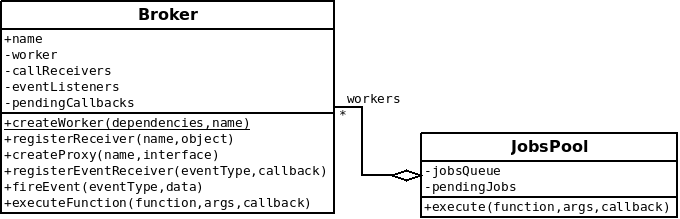
\includegraphics[scale=0.6]{zasoby/rozdzial31/broker}  
  \caption{Uproszczony diagram UML biblioteki}
  \label{fig:broker}
\end{figure}

Diagram \ref{fig:broker} przedstawia w uproszczeniu implementację omawianej biblioteki. Składa się ona
z dwóch głównych klas znajdujących się na diagramie oraz kilku mniej istotnych, które zostały pominięte
dla zachowania czytelności. Klasa Broker jest klasą najważniejszą i odpowiada za opakowanie Web Workera
w przyjazny interfejs omówiony w poprzednich podrozdziałach. Klasa JobsPool realizuje ideę puli wątków.

\section{Renderer}
\label{sec:renderer}

Renderer jest częścią silnika gry odpowiedzialną za renderowanie obiektów ze sceny gry w 3d.
Ukrywa on niskopoziomowe wywołania API graficznego (w tym przypadku WebGL) przed programistą gry.

Ponieważ WebGL jest dostępny tylko dla głównego workera, renderer ten nie może pracować na innych wątkach.
W celu osiągnięcia maksymalnej wydajności, komunikacja pomiędzy logiką gry, działającą w innym workerze,
a rendererem, została ograniczona do minimum. W tym samym celu, została ona zaprojektowana całkowicie
asynchronicznie.

\begin{figure}[h!]
  \centering
  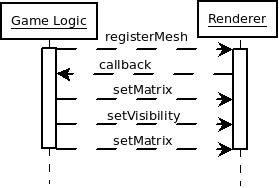
\includegraphics[scale=1]{zasoby/rozdzial31/renderer-messages}  
  \caption{Asynchroniczna komunikacja gry z rendererem}
  \label{fig:renderer-messages}
\end{figure}

Jak widać na schemacie \ref{fig:renderer-messages}, gra rejestruje na początku obiekt, który ma
być wyświetlony. Gdy rejestracja zostanie zakończona, renderer wysyła wiadomość zwrotną do gry.
Po zarejestrowaniu obiektu, renderer wyświetla go zgodnie z zapamiętanym stanem (macierz
transformacji, widoczność itd.), dopóki ten nie zostanie zmieniony.

Następnie komunikacja przepływa już tylko w jedną stronę. Gra wysyła komunikaty w celu zmiany
stanu obiektu w scenie 3d, bez oczekiwania na odpowiedź. Dzięki temu wątek gry wykonuje się
dalej podczas przekazywania i przetwarzania wiadomości. W celu dalszego zmniejszenia
narzutu wysyłania komend, są one kolejkowane po stronie gry i wysyłane większymi partiami
w jednej wiadomości.

Cały komunikacja jest opakowana w mechanizm zdalnego wywołania metod (rozdział \ref{ssec:zdalneWywolanie}),
dzięki czemu nie trzeba ręcznie tworzyć i wysyłać wiadomości. Dodatkowo, można łatwo przełączać
grę w tryb jednowątkowy w celu łatwiejszego wykrywania błędów i porównania wydajności.

\subsection{Struktura biblioteki renderera}

Diagram \ref{fig:renderer} prezentuje uproszczoną strukturę klas związanych z renderowaniem gry.

\begin{figure}[h!]
  \centering
  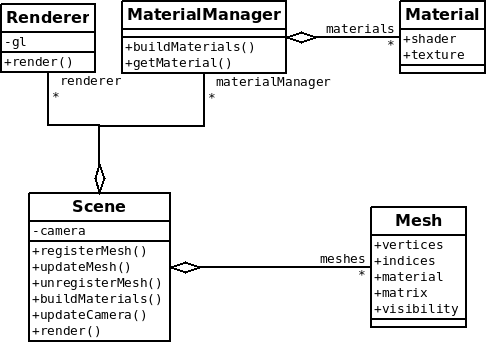
\includegraphics[scale=0.8]{zasoby/rozdzial31/renderer}  
  \caption{Uproszczony diagram klas związanych z rendererem}
  \label{fig:renderer}
\end{figure}

W następnych podrozdziałach znajduje się omówienie najważniejszych elementów biblioteki.

\subsubsection{Renderer}

Klasa o nazwie takiej samej jak nazwa całej biblioteki, odpowiada za bezpośrednią, niskopoziomową
komunikację z WebGL. Pośredniczy ona pomiędzy wysokopoziomową klasą sceny, operującej na
pojęciach obiektów, ich materiałów i pozycji, a niskopoziomowym API do rysowania trójkątów
za pomocą shaderów. Klasa renderera potrzebuje stanu obiektu, który otrzymuje od sceny
oraz materiał\footnote{Materiał graficzny -- zbiór właściwości opisujących wygląd obiektu, takich jak
kolor, tekstura, shader wykorzystywany do renderowania itp.}, przechowywany w menedżerze materiałów.

\subsubsection{Scena}

Klasą, która zarządza całym modułem renderera jest scena. Przechowuje ona stan wszystkich
zarejestrowanych przez grę obiektów graficznych oraz bezpośrednio odbiera i wykonuje
komendy zmiany stanu obiektu wysłane przez grę.

Po wywołaniu funkcji renderującej, scena przekazuje do niskopoziomowej klasy renderera
stan wszystkich obiektów razem z potrzebnymi

\subsubsection{Menedżer materiałów}

Do zadań menedżera materiałów należy tworzenie, przechowywanie i zarządzanie materiałami
graficznymi. Podczas inicjalizacji gry, menedżer tworzy potrzebne materiały. Podczas
ich tworzenia, konieczne jest między innymi wysłanie tekstur do pamięci karty graficznej
za pośrednictwem WebGL, a także skompilowanie używanych shaderów. Klasa ta dba również
o to, aby materiały nie dublowały się, zajmując niepotrzebnie pamięć.

\section{Zasoby gry}
\label{sec:zasobyGry}

WebArena wykorzystuje wiele rodzajów zasobów potrzebnych do wyświetlania grafiki i sterowania
logiką gry. Są to następujące pliki:
\begin{itemize}
\item pliki bsp z opisami poziomów gry,
\item pliki md3 z modelami 3d postaci, broni i innych przedmiotów,
\item opisy materiałów graficznych,
\item tekstury,
\item różnorakie pliki konfiguracyjne.
\end{itemize}

W związku z tym, że WebArena wykorzystuje zasoby gry OpenArena, wszystkie pliki są zgodne
z formatem używanym przez Quake III Arena. W dalszych podrozdziałach nastąpi omówienie
kodu odpowiedzialnego za wczytywanie zasobów wraz z pobieżnym omówieniem formatów plików.

\begin{figure}[h]
  \centering
  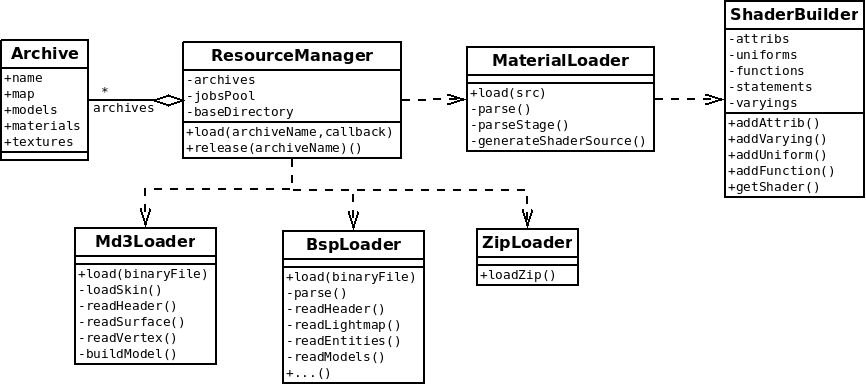
\includegraphics[scale=0.5]{zasoby/rozdzial31/resources}  
  \caption{Uproszczony diagram klas związanych z zarządzaniem zasobami.}
  \label{fig:screen}
\end{figure}

\subsection{Pliki BSP}

Pliki BSP służą do opisu geometrii i wyglądu poziomu. Format ten wywodzi się z Quake III. Nazwa
BSP oznacza Binary Space Partitioning i jest to również nazwa struktury danych (drzewo BSP),
w którym przechowywana jest geometria całego poziomu.
Drzewo BSP przyśpiesza wiele operacji wykonywanych w trakcie gry, a przede wszystkim wykrywanie
kolizji gracza lub pocisku z przedmiotami w świecie gry.

Kolejną ważną cechą plików BSP jest przechowywanie tzw. lightmapy, która służy do przedstawiania
realistycznego oświetlenia poziomu.

Plik BSP dzieli się na kilkanaście sekcji, przechowujących między innymi informacje o:
\begin{itemize}
\item budowie drzewa BSP,
\item wierzchołkach,
\item materiałach graficznych,
\item lightmapie,
\item efektach (takich jak np. mgła).
\end{itemize}

Dokładną specyfikację pliku BSP można znaleźć na na stronie \cite{bsp}. W WebArena do parsowania
pliku został częściowo wykorzystany kod z dema Brandona Jonesa opisanego w rozdziale \ref{ssec:quake3web}.

Ponieważ parsowanie pliku jest czasochłonne, jego wykonanie odbywa się na osobnym
wątku za pośrednictwem biblioteki opisanej w rozdziale \ref{sec:wielowatkowosc}.

\subsection{Pliki MD3}

MD3 jest formatem plików modeli graficznych używanym przez Quake III Arena. W plikach tych przechowywane
są wszystkie ruchome modele, takie jak postacie, bronie itp.

Ich ważną cechą jest możliwość przechowywania
animacji (w przeciwieństwie do plików BSP). Jest to animacja wierzchołkowa, w której dla każdej klatki
animacji, przechowywane są pozycje wszystkich wierzchołków. Sposób ten powoduje duże zużycie pamięci,
jednak jego zaletą jest prostota.

Kod do wczytywania plików MD3 został napisany specjalnie dla WebArena w oparciu o specyfikację dostępną 
na stronie \cite{md3} i tak jak w przypadku BSP, wykonywany jest na osobnym wątku.

\subsection{Pliki materiałów graficznych i tekstury}

Quake III Arena powstał w czasach gdy jeszcze niemożliwe było tworzenie shaderów. Na karcie graficznej
mógł działać tylko predefiniowany przez producenta program do renderowania, można było sterować jedynie
jego parametrami. Był to tzw. fixed pipeline.

Aby obejść ograniczenia tego rozwiązania i umożliwić grafikom elastyczne definiowanie wyglądu
powierzchni, id Tech 3 wprowadził pliki tekstowe z opisem materiałów graficznych, częściowo pełniących
również rolę dzisiejszych shaderów. Pliki te również były nazywane shaderami, co może wprowadzać
pewną niejasność, dlatego w tej pracy konsekwentnie będzie używane pojęcie materiału.

\begin{lstlisting}[caption=Przykładowy opis materiału]
models/powerups/ammo/machammo
{
	{
		map models/powerups/ammo/ammobox.tga
		rgbGen lightingDiffuse
	}
	{
		map models/powerups/ammo/ammolights.tga
		blendfunc blend
		rgbGen const ( 1 1 0 )
		alphaGen wave sawtooth 0 1 0 1 
	}
}
\end{lstlisting}

Dokładną specyfikację plików materiałów można znaleźć w \cite{q3shaders}.

Ponieważ przestarzały fixed pipeline jest całkowicie usunięty z OpenGL ES i WebGL, dlatego konieczne
było przetłumaczenie materiałów na kod shadera. Jest to realizowane podczas wczytywania materiału.
Większość kodu wczytującego i tłumaczącego materiały jest pobrane z pracy Brandona Jonesa (rozdział
\ref{ssec:quake3web}).

\subsection{Menedżer zasobów}

Menedżer zasobów zarządza wczytywaniem i przechowaniem zasobów z pomocą wyżej wymienionych parserów.
Wszystkie pliki wczytywane są asynchronicznie, za pomocą puli wątków opisanej w rozdziale \ref{ssec:puleWatkow}.
Dzięki temu interfejs użytkownika nie blokuje się nawet podczas wczytywania bardzo dużych plików.
Menedżer dba również, aby żaden plik nie został wczytany dwukrotnie, co oznaczałoby marnowanie
pamięci.

W przypadku gry sieciowej nie można pominąć kwestii przesyłania plików przez internet. Wszystkie
zasoby muszą być pobrane z serwera przed rozpoczęciem rozgrywki. Konieczne jest jednak maksymalne
skrócenie czasu oczekiwania gracza.

Ściąganie każdego pliku osobno jest bardzo nieefektywne, z drugiej jednak strony pobieranie wszystkich
zasobów w jednym dużym archiwum trwało by zbyt długo. Dlatego trzeba podzielić pliki na kilka
archiwów, tak aby gracz pobierał jedynie te potrzebne do zagrania w dany poziom.

W tym celu został napisany skrypt działający po stronie serwera, który analizuje plik BSP lub MD3 i pakuje
go do jednego archiwum zip razem z wszystkimi plikami, do których się odwołuje (materiały, tekstury,
modele). Dzięki temu gra pobiera jedynie kilka plików zip, które są po stronie przeglądarki rozpakowywane.

Komunikacja odbywa się za pomocą technologii AJAX\footnote{AJAX (Asynchronous JavaScript and XML) -- technologia
służąca do wykonywania asynchronicznych zapytań HTML z języka JavaScript.}.

\section{Synchronizacja sieciowa}
\label{sec:synchronizacjaSieciowa}

Jedną z najciekawszych części projektu jest biblioteka służąca do synchronizacji stanu gry pomiędzy
komputerami w sieci. Biblioteka napisana jest w taki sposób, aby łatwo można jej było użyć w innych
projektach.

Ręczne pisanie kodu do synchronizacji danych jest bardzo żmudnym zadaniem. Trzeba pamiętać o wielu
niskopoziomowych problemach, takich jak zgubione pakiety (przez zawodny protokół UDP), czy
też zbyt duży ich rozmiar. Dlatego istotne jest wprowadzenie mechanizmu, który zautomatyzuje synchronizację.
W idealnym rozwiązaniu, programista gry wskazuje jedynie które pola w poszczególnych obiektach
powinny być przesyłane, dając również wskazówki np. co do wymaganej dokładności, czy częstotliwości
synchronizacji. Taki sposób programowania jest zgodny z paradygmatem programowania deklaratywnego,
w którym programista określa jaki cel chce osiągnąć, a nie musi podawać sposobu na jego osiągnięcie.

Biblioteka do synchronizacji powinna więc spełniać następujące założenia:
\begin{itemize}
\item prostota użycia,
\item zwolnienie programisty gry z konieczności pamiętania o niskopoziomowych problemach komunikacji
  sieciowej,
\item możliwość rekurencyjnego synchronizowania całych drzew obiektów,
\item kompresja różnicowa (przesyłanie jedynie zmian stanu) dla zmniejszenia rozmiarów danych,
\item bezproblemowe działanie w warunkach często traconych pakietów.
\end{itemize}

\subsection{Sposób użycia biblioteki}

Na listingu \ref{lst:uzycie} przedstawiono kod synchronizujący jeden z obiektów gry -- jest
to obiekt reprezentujący postać gracza. Pozostałe funkcje tego obiektu nie są teraz istotne.

\begin{lstlisting}[label=lst:uzycie,caption=Kod synchronizujący jeden z obiektów gry]
/**
 * @public
 * @param {network.ISynchronizer} sync
 */
game.Player.prototype.synchronize = function (sync) {
    // poniższe trzy obiekty zostaną zsynchronizowane rekurencyjnie
    this.head = sync.synchronize(this.head, Type.OBJECT);
    this.torso = sync.synchronize(this.torso, Type.OBJECT);
    this.legs = sync.synchronize(this.legs, Type.OBJECT);

    // INT8 określa typ i wymaganą dokładność (8 bitów)
    this.legsState = sync.synchronize(this.legsState, Type.INT8);
    this.torsoState = sync.synchronize(this.torsoState, Type.INT8);

    this.lastYaw = sync.synchronize(this.lastYaw, Type.FLOAT32);
    this.legsAngle = sync.synchronize(this.legsAngle, Type.FLOAT32);
};
\end{lstlisting}

Każdy obiekt, który ma być synchronizowany musi definiować funkcję \emph{synchronize}, która jako
argument przyjmuje obiekt synchronizatora (przedstawiony w następnym podrozdziale). Synchronizacja jest
przemyślana w taki sposób, aby nie było konieczne pisanie osobnych funkcji odczytujących i zapisujących
(choć jest to możliwe w razie konieczności).
Dzięki temu unika się błędów związanych z różną kolejnością zapisu i odczytu składowych lub pominięcia
jednej z nich.

Synchronizator pamięta czy pracuje w trybie odczytu i zapisu. Jeśli jest to tryb odczytu,
jego funkcja \emph{synchronize} zwraca dokładnie taką wartość jaką otrzymała i obiekt pozostaje niezmieniony.

Jak widać, możliwa jest synchronizacja nie tylko typów prostych, ale również obiektów zdefiniowanych
przez użytkownika. Dzięki temu można jednym wywołaniem zapisać i odczytać całą scenę gry.

\section{Omówienie struktury biblioteki}

\begin{figure}[h!]
  \centering
  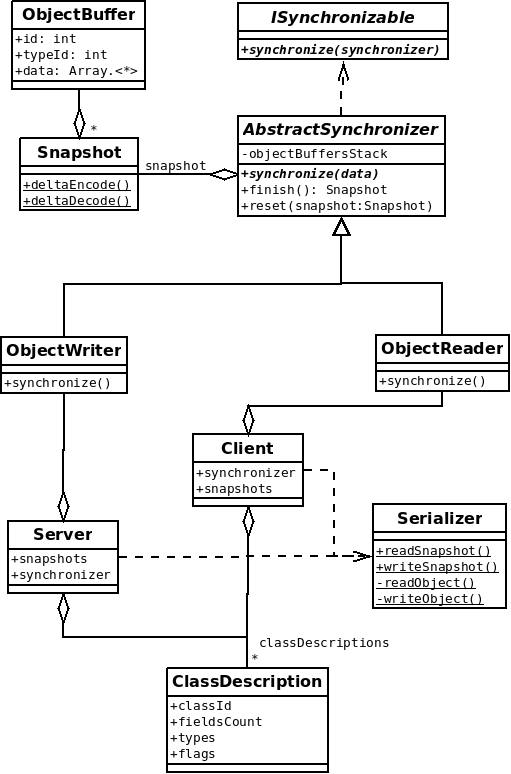
\includegraphics[scale=0.7]{zasoby/rozdzial31/network}  
  \caption{Diagram klas biblioteki do synchronizacji sieciowej.}
  \label{fig:networkSync}
\end{figure}

Rysunek \ref{fig:networkSync} przedstawia diagram klas biblioteki.
Najważniejszą klasą jest \emph{AbstractSynchronizer}, z której dziedziczą odpowiednio \emph{ObjectReader}
i \emph{ObjectWriter}. \emph{ObjectReader} jest przekazywany odczytywanym obiektom do funkcji \emph{synchronize},
zaś \emph{ObjecWriter}, jest używany podczas zapisywania obiektu.

Każdy obiekt który ma być synchronizowany, musi implementować interfejs \emph{ISynchronizable}\footnote{
  Oczywiście, z racji tego, że JavaScript jest językiem dynamicznym i nie ma w nim pojęcia interfejsu,
  mowa tu tylko o implementacji interfejsu w sensie koncepcyjnym. Z punktu widzenia języka, wystarczy
  jeśli dany obiekt posiada odpowiednie metody.}.

Całym procesem synchronizacji sterują klasy \emph{Client} lub \emph{Server}, w zależności od tego, czy
gra działa jako klient czy serwer. Dodatkowe klasy zajmują się przechowywaniem całego stanu gry, kompresją
różnicową oraz serializacją stanu do postaci binarnej.

\section{Logika gry}
\label{sec:logikaGry}

Kod sterujący logiką korzysta z wszystkich wyżej wymienionych komponentów. Działa równolegle do kodu renderera,
na osobnym wątku. Ma swoją pętlę główną, podczas której następuje synchronizacja sieciowa, aktualizacja stanu gry,
oraz przesłanie aktualizacji stanu do renderera. Jej implementacja jest zgodna z opisem z rozdziału
\ref{ssec:petlaGlowna}, z jedną tylko istotną różnicą -- logika gry nie uruchamia renderowania, a jedynie
przesyła do wątku renderera (który cały czas renderuje świat gry) aktualizację stanu.

Tradycyjnie do implementacji logiki gry często używa się języków skryptowych, które są bardziej przystępne 
i elastyczne od języków natywnych oraz umożliwiają szybką aktualizację kodu w czasie działania gry, co znacząco
wpływa na szybkość jej tworzenia. Takie rozwiązanie ma jednak wadę w postaci konieczności osadzenia
w grze wirtualnej maszyny i udostępnienia dla niej odpowiedniego API. W przypadku JavaScript, cała
gra jest napisana w języku skryptowym, nie ma więc konieczności dodawania drugiego języka i tworzenia
warstwy pośredniczącej.

\subsection{Omówienie struktury}
\begin{figure}[h]
  \centering
  \includegraphics[scale=0.4]{zasoby/rozdzial31/game}  
  \caption{Diagram klas przedstawiający logikę gry}
  \label{fig:gameClasses}
\end{figure}

Diagram \ref{fig:gameClasses} przedstawia strukturę klas składających się na stan gry. Wszystkie obiekty
znajdujące się w świecie gry wywodzą się z klasy \emph{EntityState}. Do obiektów tych należą:
\begin{itemize}
\item gracze (\emph{PlayerState}),
\item pociski, takie jak rakiety (\emph{ProjectileState}),
\item przedmioty, które gracze mogą zbierać, takie jak bronie, amunicja, apteczki (\emph{ItemState}).
\end{itemize}

Postać gracza jest podzielona na trzy części (\emph{PlayerPartState}) -- głowę, tułów i nogi, z których
każda animuje się oddzielnie. Dzięki temu możliwe jest jednoczesne bieganie w dowolnym kierunku
i strzelanie. Nie wszystkie możliwości, które daje przedstawiona struktura zostały wykorzystane w aktualnej
wersji gry. Na razie nie ma jeszcze przedmiotów do podnoszenia oraz rakiet, jednak przy istniejącym
kodzie ich dodanie jest już łatwym zadaniem.


\section{Opis z punktu widzenia użytkownika}

Gotową grę można zobaczyć na stronie \url{http://game-webarena.rhcloud.com/}.

Po wejściu na stronę, automatycznie uruchamiana jest gra w trybie serwera. Generowany jest też link,
który można przesłać znajomemu, chcącemu dołączyć do gry. Po wejściu w podany URL, zostanie on podłączony
do gry jako klient.

Sterowanie jest bardzo podobne do innych gier typu FPS:
\begin{itemize}
\item mysz -- rozglądanie się,
\item lewy przycisk myszy -- strzał,
\item spacja -- skok,
\item W, S, A, D -- poruszanie się (odpowiednio: do przodu, do tyłu, lewo, prawo),
\item ctrl -- kucnięcie.
\end{itemize}

Gra działa na przeglądarkach Google Chrome i Mozilla Firefox w najnowszych wersjach. Obsługa innych
przeglądarek może zostać dodana, kiedy będą już miały zaimplementowaną obsługę wszystkich potrzebnych
standardów i wystarczająco szybki silnik JavaScript.

Grafika \ref{fig:screen} przedstawia zrzut ekranu z gry.

\begin{figure}[h]
  \centering
  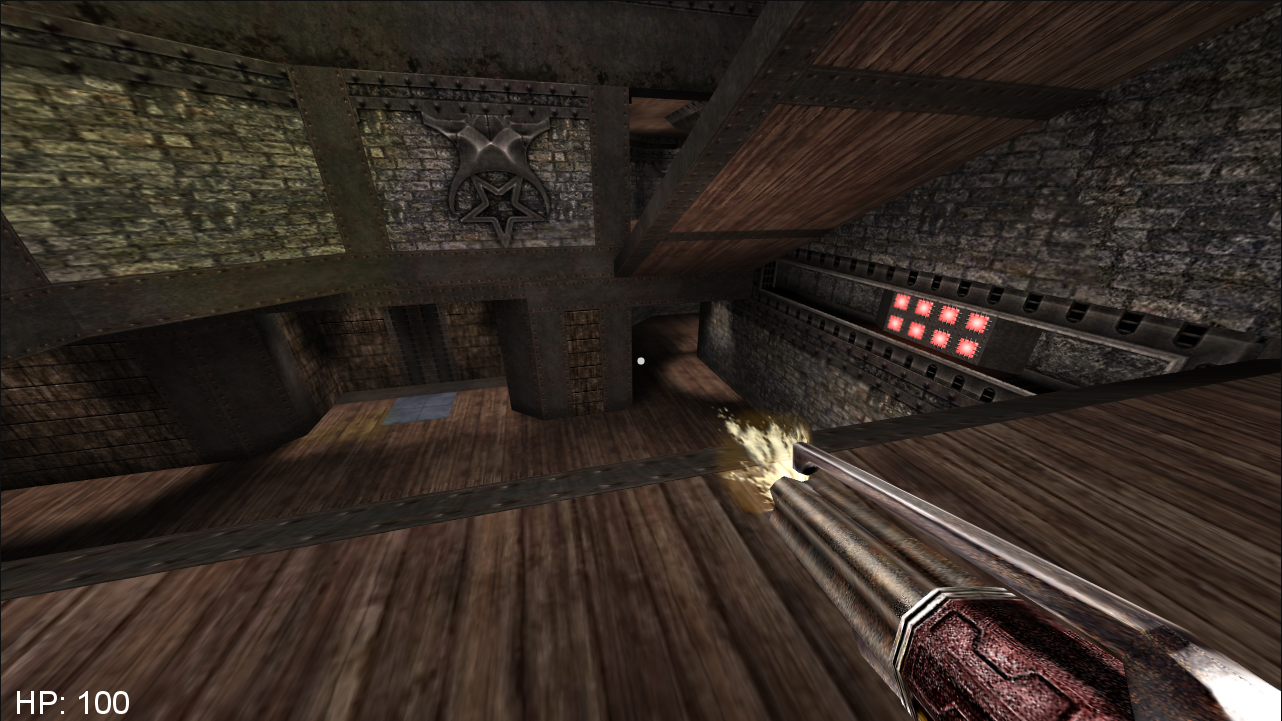
\includegraphics[scale=0.45]{zasoby/rozdzial31/screen}  
  \caption{Zrzut ekranu z gry Web Arena}
  \label{fig:screen}
\end{figure}


%%% Local Variables: 
%%% mode: latex
%%% TeX-master: "praca"
%%% End: 

\chapter{Analiza}


%%% Local Variables: 
%%% mode: latex
%%% TeX-master: "praca"
%%% End: 

\chapter{Podsumowanie}
\label{cha:podsumowanie}

Nowe technologie związane z HTML 5 stwarzają dla twórców gier szansę zdobycia nowych rynków.
Niniejsza praca miała na celu zbadanie tematu tworzenia gier w HTML 5, na przykładzie gry
typu FPS.
Podczas pisania pracy udało się stworzyć projekt, odtwarzający jedną ze znanych gier
w przeglądarce internetowej.


\section{Ocena realizacji celów pracy}
Praca miała następujące cele:
\begin{enumerate}
\item Stworzenie gry typu FPS z wykorzystaniem technologii zawartych w HTML 5.
\item Analiza możliwości tych technologii w porównaniu do tradycyjnego podejścia do tworzenia gier.
\end{enumerate}

Cele te udało się zrealizować.

Realizację celu pierwszego można śledzić w rozdziałach \ref{cha:projekt} i \ref{cha:implementacja}.
Cel drugi został zrealizowany w rozdziale \ref{cha:analiza}.


\section{Ocena prawdziwości tezy pracy}

Niniejsza praca dowodzi prawdziwości tezy:
\emph{Technologia HTML 5 umożliwia tworzenie zaawansowanych gier 3D.}

\section{Możliwości dalszego rozwoju projektu}
\label{sec:mozliwosciRozwoju}

O ile projekt realizuje badawczy cel pracy, o tyle prezentuje raczej poziom technologicznego
eksperymentu niż produktu komercyjnego. Możliwe jest jednak rozbudowanie go, aby nadawał się
do upublicznienia w internecie. Oto potencjalne kierunki rozwoju gry:

\begin{itemize}
\item ulepszenie i optymalizacja renderera,
\item dodanie nowych broni i przedmiotów do gry,
\item nowe poziomy,
\item nowe tryby gry (np. drużynowy),
\item nowe modele postaci,
\item integracja z portalami społecznościowymi,
\item rankingi graczy,
\item system zabezpieczający przed oszukiwaniem w rozgrywce sieciowej,
\item wprowadzenie opcjonalnych płatności za dodatkową zawartość w grze.
\end{itemize}



%%% Local Variables: 
%%% mode: latex
%%% TeX-master: "praca"
%%% End: 


% itd.
%\appendix
%\chapter{Użyte narzędzia}
\label{cha:uzyteNarzedzia}

\section{Google Closure}
\label{sec:googleClosure}

%%% Local Variables: 
%%% mode: latex
%%% TeX-master: "praca"
%%% End: 

% \include{dodatekB}
% itd.

\bibliographystyle{abbrv}
\bibliography{bibliografia}
%\begin{thebibliography}{1}
%
%\bibitem{Dil00}
%A.~Diller.
%\newblock {\em LaTeX wiersz po wierszu}.
%\newblock Wydawnictwo Helion, Gliwice, 2000.
%
%\bibitem{Lam92}
%L.~Lamport.
%\newblock {\em LaTeX system przygotowywania dokumentów}.
%\newblock Wydawnictwo Ariel, Krakow, 1992.
%
%\bibitem{Alvis2011}
%M.~Szpyrka.
%\newblock {\em {On Line Alvis Manual}}.
%\newblock AGH University of Science and Technology, 2011.cccccc
%\newblock \\\texttt{http://fm.ia.agh.edu.pl/alvis:manual}.
%
%\end{thebibliography}

\end{document}

%%% Local Variables: 
%%% mode: latex
%%% TeX-master: t
%%% End: 
